\chapter{Introduction}
\label{chapter:Introduction}

\section{Types of machine learning}
\begin{equation}\nonumber
\begin{cases}
\text{Supervised Learning} \begin{cases} \text{Classification} \\ \text{Regression} \end{cases}\\
\text{Unsupervised Learning} \begin{cases} \text{Discovering clusters} \\ \text{Discovering latent factors} \\ \text{Discovering graph structure} \\ \text{Matrix completion} \end{cases}\\
\text{Reinforcement Learning}
\end{cases}
\end{equation}
In the \textbf{predictive} or \textbf{supervised learning} approach,the goal is to learn a \textbf{mapping} from \textbf{inputs} $\mathbf{x}$ to \textbf{outputs} $y$,given a labeled set of input-output paris $D=\{(\mathbf{x_i},y_i)\}_{i=1}{N}$.Here $D$ is called the \textbf{training set},and N is the number of training examples.
In the simplest setting,each training input $\mathbf{x_i}$ is a D-dimensional vector of numbers,representing,say,the height and weight of a person,which are called \textbf{features,attributes,or covariates}.

\section{Supervised learning}
  Similarly the form of the output or \textbf{response variable} can in principle be anything,but most methods assume that $y_i$ is \textbf{categorical or nominal} variable from some finite set,$y_i \in \{1,...,C\}$.When $y_i$ is categorical,the problem is known as \textbf{classification or pattern recognition},and when real-valued,known as \textbf{regression}.
\subsection{Classification}
  Here the goal is to learn a mapping from inputs $x$ to outputs $y$,where $y \in \{1,...,C\}$,with $C$ being the number of classes.If $C=2$,this is called \textbf{binary classification};if $C>2$,this is called \textbf{multiclass classification}.if the class labels are not mutually exclusive,we call it \textbf{multi-label classification},but this is best viewed as predicting multiple related binary class labels(a so-called \textbf{multiple output model}).
  One way to formalize the problem is as \textbf{function approximation}:assume $y=f(\mathbf{x})$ for some unknown function $f$,and the goal of learning is to estimate the function $f$ given a labeled training set,and then to make predictions(estimate) using $\hat{y} =\hat{f}(\mathbf{x})$.Our main goal is to make predictions on novel inputs,meaning ones that we have not seen before(\textbf{generalization}.
\subsubsection{Probabilistic predictions}
We denote the probability distribution over possible labels,given the input vector $\vec{x}$ and training set $\mathcal{D}$ by $p(y|\vec{x},\mathcal{D})$.
Given a probabilistic output,we can always compute out "best guess" as to the "true label" using
\begin{equation}
\hat{y} = \hat{f}(\mathbf{x}) = \arg\max\limits_{c=1}^{C} p(y=c|\mathbf{x},D)
\end{equation}
This corresponds to the most probable class label,and is called the \textbf{mode} of distribution $p(y|\vec{x},\mathcal{D})$;it is also known as a \textbf{MAP estimate}(MAP stands for\textbf{maximum a posteriori}).
\subsubsection{Applications}
\subsection{Regression}

\section{Unsupervised learning}
  \textbf{Descriptive or unsupervised learning} approach is sometimes called \textbf{knowledge discovery}.We will formalize out task as one of \textbf{density estimation},that is we want to build models of the form $p(\mathbf{x_i|\theta})$,instead of $p(y_i|\mathbf{x_i,\theta})$.
\subsection{Discovering clusters}
Let $z_i \in \{1,...,K\}$ represent the cluster to which data point $i$ is assigned.($z_i$ is an exmaple of \textbf{hidden or latent} variable).
\subsection{Discovering latent factors}
Although the data may appear high dimensional,there may only be a small number of degrees of variability,corresponding to \textbf{latent factors}.The most common approach to dimensionality reduction is called \textbf{principal components analysis or PCA}.
\subsection{Discovering graph structure}
\subsection{Matrix completion}
\subsubsection{Image inpainting}
\subsubsection{Collaborative filtering}
\subsubsection{Market basket analysis}

\section{Three elements of a machine learning model}

\textbf{Model = Representation + Evaluation + Optimization}\footnote{Domingos, P. A few useful things to know about machine learning. Commun. ACM. 55(10):78–87 (2012).}


\subsection{Representation}
In supervised learning, a model must be represented as a conditional probability distribution $P(y|\vec{x})$(usually we call it classifier) or a decision function $f(x)$. The set of classifiers(or decision functions) is called the hypothesis space of the model. Choosing a representation for a model is tantamount to choosing the hypothesis space that it can possibly learn. 


\subsection{Evaluation}
In the hypothesis space, an evaluation function (also called objective function or risk function) is needed to distinguish good classifiers(or decision functions) from bad ones.


\subsubsection{Loss function and risk function}
\label{sec:Loss-function-and-risk-function}

\begin{definition}
In order to measure how well a function fits the training data, a \textbf{loss function} $L:Y \times Y \rightarrow R \geq 0$ is defined. For training example $(x_i,y_i)$, the loss of predicting the value $\widehat{y}$ is $L(y_i,\widehat{y})$.
\end{definition}

The following is some common loss functions:
\begin{enumerate}
\item 0-1 loss function \\ $L(Y,f(X))=\mathbb{I}(Y,f(X))=\begin{cases} 1, & Y=f(X) \\ 0, & Y \neq f(X) \end{cases}$
\item Quadratic(squared) loss function $L(Y,f(X))=\frac{1}{2}\left(Y-f(X)\right)^2$
\item Absolute loss function $L(Y,f(X))=\abs{Y-f(X)}$
\item Exponential loss function $L(Y,f(X)=exp(-\hat{y_i}f(\mathbf{x_i}))$ 
\item Logarithmic loss function \\ $L(Y,P(Y|X))=-\log{P(Y|X)}$
\end{enumerate}

\begin{tabular}{l*{3}{c}r}
Name & Loss & Derivative & $f^*$ & Algorithm                                                                                 \\
\hline
Squared error & $\frac{1}{2}(y_i-f(\mathbf{x_i}))^2$ & $y_i - f(\mathbf{x_i})$ & $\mathbb{E}[y|\mathbf{x_i}]$ & L2Boosting \\
Absolute error & $|y_i-f(\mathbf{x_i})|$ & $sgn(y_i-f(\mathbf{x_i}))$ & $median(y|\mathbf{x_i})$ & Gradient boosting \\
Exponential loss & $exp(-\hat{y_i}f(\mathbf{x_i}))$ & $-\hat{y_i}exp(-\hat{y_i}f(\mathbf{x_i}))$ & $\frac{1}{2}log\frac{\pi_i}{1-\pi_i}$ & AdaBoost \\
Logloss & $log(1+e^{-\hat{y_i}f_i})$ & $y_i-\pi_i$ & $\frac{1}{2}log\frac{\pi_i}{1-\pi_i•}$ & LogitBoost \\
\hline
\end{tabular}

\begin{definition}
The risk of function $f$ is defined as the expected loss of $f$:
\begin{equation}\label{eqn:expected-loss}
R_{\mathrm{exp}}(f)=E\left[L\left(Y,f(X)\right)\right]=\int L\left(y,f(x)\right)P(x,y)\mathrm{d}x\mathrm{d}y
\end{equation}
which is also called expected loss or \textbf{risk function}.
\end{definition}

\begin{definition}
The risk function $R_{\mathrm{exp}}(f)$ can be estimated from the training data as
\begin{equation}
R_{\mathrm{emp}}(f)=\dfrac{1}{N}\sum\limits_{i=1}^{N} L\left(y_i,f(x_i)\right)
\end{equation}
which is also called empirical loss or \textbf{empirical risk}.
\end{definition}

You can define your own loss function, but if you're a novice, you're probably better off using one from the literature. There are conditions that loss functions should meet\footnote{\url{http://t.cn/zTrDxLO}}:
\begin{enumerate}
\item They should approximate the actual loss you're trying to minimize. As was said in the other answer, the standard loss functions for classification is zero-one-loss (misclassification rate) and the ones used for training classifiers are approximations of that loss.
\item The loss function should work with your intended optimization algorithm. That's why zero-one-loss is not used directly: it doesn't work with gradient-based optimization methods since it doesn't have a well-defined gradient (or even a subgradient, like the hinge loss for SVMs has).

The main algorithm that optimizes the zero-one-loss directly is the old perceptron algorithm(chapter \S \ref{chap:Perceptron}).
\end{enumerate}


\subsubsection{ERM and SRM}
\begin{definition}
ERM(Empirical risk minimization)
\begin{equation}
\min\limits _{f \in \mathcal{F}} R_{\mathrm{emp}}(f)=\min\limits _{f \in \mathcal{F}} \dfrac{1}{N}\sum\limits_{i=1}^{N} L\left(y_i,f(x_i)\right)
\end{equation}
\end{definition}

\begin{definition}
Structural risk
\begin{equation}
R_{\mathrm{smp}}(f)=\dfrac{1}{N}\sum\limits_{i=1}^{N} L\left(y_i,f(x_i)\right) +\lambda J(f)
\end{equation}
\end{definition}

\begin{definition}
SRM(Structural risk minimization)
\begin{equation}
\min\limits _{f \in \mathcal{F}} R_{\mathrm{srm}}(f)=\min\limits _{f \in \mathcal{F}} \dfrac{1}{N}\sum\limits_{i=1}^{N} L\left(y_i,f(x_i)\right) +\lambda J(f)
\end{equation}
\end{definition}


\subsection{Optimization}
Finally, we need a \textbf{training algorithm}(also called \textbf{learning algorithm}) to search among the classifiers in the the hypothesis space for the highest-scoring one. The choice of optimization technique is key to the \textbf{efficiency} of the model.

\section{Model Selection}
If data is plentiful,then on approach to avoid over-fitting is to use some of the some of the available data to train a range of models,or a given model with a range of values for its complexity parameters,and then to compare them on independent data,sometimes called a \textbf{Validation set},and select the one having the best predictive performance.If the model design is iterated many times using a limited size data set,then some over-fitting to the validation data can occur and so it may be necessary to keep aside a third \textbf{test set} on which the performance of the selected model is finally evaluated.

\subsubsection{Cross validation}
\label{sec:Cross-validation}
\begin{definition}
	\textbf{Cross validation}, sometimes called \emph{rotation estimation}, is a \emph{model validation} technique for assessing how the results of a statistical analysis will generalize to an independent data set\footnote{\url{http://en.wikipedia.org/wiki/Cross-validation_(statistics)}}.
\end{definition}

Common types of cross-validation:
\begin{enumerate}
	\item K-fold cross-validation. In k-fold cross-validation, the original sample is randomly partitioned into k equal size subsamples. Of the k subsamples, a single subsample is retained as the validation data for testing the model, and the remaining k − 1 subsamples are used as training data.
	\item 2-fold cross-validation. Also, called simple cross-validation or holdout method. This is the simplest variation of k-fold cross-validation, k=2.
	\item Leave-one-out cross-validation(\emph{LOOCV}). k=M, the number of original samples.
\end{enumerate}
In many applications,however,the supply of data for training and testing will be limited.We wish to use as much of available data as possible for both training and validation set.One solution to this dilemma is to use \textbf{cross-validations}.One round of cross-validation involves partitioning a sample of data into complementary subsets, performing the analysis on one subset (called the training set), and validating the analysis on the other subset (called the validation set or testing set). To reduce variability, multiple rounds of cross-validation are performed using different partitions, and the validation results are averaged over the rounds.


\section{The Curse of Dimensionality}
The common theme that arise when analyzing and organizing data in \textbf{high-dimensional spaces} is that when the \textbf{demensionality increases},the \textbf{volume of the space} increases so fast (\textbf{grows exponentially with the dimensionality}) that the available data become sparse.

\begin{figure}
	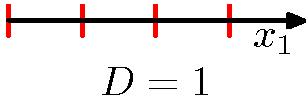
\includegraphics[ ]{figures/prml/Figure1.21a.jpg}
	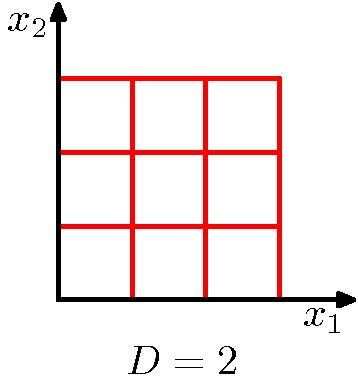
\includegraphics[ ]{figures/prml/Figure1.21b.jpg}
	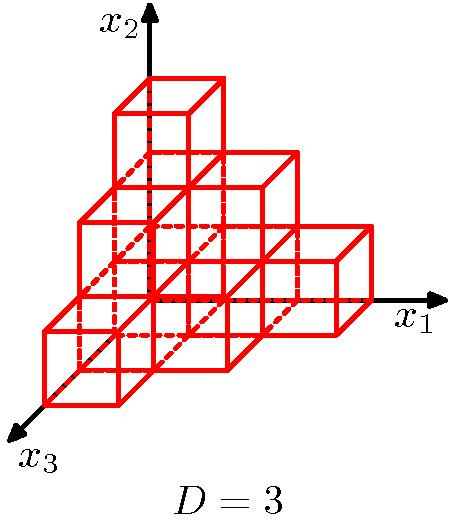
\includegraphics[ ]{figures/prml/Figure1.21c.jpg}
	\caption{Illustration of the curse of dimensionality:the number of regions of a regular grid grows exponentially with the dimensionality $D$ of the space.}
\end{figure}
The volume of a sphere of radius $r$ in $D$ dimensions must scale as $r^D$,and so we write
\begin{align}
V_D(r) = K_D r^D
\end{align}
The fraction of the volume of the sphere that lies between radius $r=1-\epsilon$ and $r=1$
\begin{align}
\dfrac{V_D(1)-V_D(1-\epsilon)}{V_D(1)}=1-(1-\epsilon)^D
\end{align}
for large $D$ this fraction tends to $1$ even for small values of $\epsilon$.Thus most of the volume of a sphere is concentrated in a thin shell near the surface!

\section{Decision Theory}
Probability theory provides us with a consistent mathematical framework for quantifying and manipulating uncertainty.And when combined with probability theory,decision theory allows us to make optimal decisions in situations involving uncertainty such as those encountered in pattern recognition.

Suppose we have an input vector x together with a corresponding vector t of target variables, and our goal is to predict t given a new value for x. For regression problems, t will comprise continuous variables, whereas for classification problems t will represent class labels. The joint probability distribution p(x, t) provides a complete summary of the uncertainty associated with these variables. Determination of p(x, t) from a set of training data is an example of \textbf{inference} and is typically a very difficult problem.

The \textbf{decision} step, is the subject of decision theory to tell us how to make optimal decisions given the appropriate probabilities. We shall see that the decision stage is generally very simple, even trivial, once we have solved the inference problem.

Consider,for a classification problem,in which case,the input are vectors  $\vec{x}$ and we denote the class $i$ by $\mathcal{C}_k$.Using Bayes' theorem,these probabilities can be expressed in the form
\begin{equation}
p(\mathcal{C}_k|\vec{x}) = \dfrac{p(\vec{x}|\mathcal{C}_k)p(\mathcal{C}_k)}{p(\vec{x})}
\end{equation}
Note that any of the quantities appearing in Bayes' theorem can be obtained from the joint distribution $p(\vec{x},\mathcal{C}_k)$ by either \textbf{marginalizing} or \textbf{conditioning} with respect to the appropriate variables.We can now interpret $p(\mathcal{C}_k)$ as the prior probability for the class $\mathcal{C}_k$,and the $p(\mathcal{C}_k|\vec{x})$ as the corresponding posterior probability,$p(\vec{x}|\mathcal{C}_k)$ is the likelihood function.If our aim it to minimize the chance of assigning $\vec{x}$ to the wrong class,then intuitively we would choose the class having the higher posterior probability.
\subsection{Minimizing the misclassification rate}
\subsection{Minimizing the expected loss}
\subsection{The reject option}
\subsection{Inference and decision}
We have broken the classification problem down into two separate stages,the \textbf{inference stage} in which we use training data to learn to \textbf{model} for $p(\mathcal{C}_k|\vec{x})$,and the subsequent \textbf{decision stage} in which we use these posterior probabilities to make optimal class assignments.An alternative  possibility would be to solve both problems together and simply learn a function that maps input $\vec{x}$ directly into decisions.Such a function is called a \textbf{discriminant function}.

In fact,we can identify three distinct approaches to solving decision problems,given, in decreasing order of complexity,by
\begin{enumerate} %[label=(\alph*)]
	\item First solve the inference problem of determining the class-conditional densities
	$p(x|\mathcal{C}_k)$ for each class $\mathcal{C}_k$ individually. Also separately infer the prior class probabilities $p(\mathcal{C}_k)$. Then use $Bayes’$ theorem in the form 
	\begin{equation}
	p(\mathcal{C}_k|\vec{x}) = \dfrac{p(x|\mathcal{C}_k)p(\mathcal{C}_k)}{p(\vec{x})}
	\end{equation}
	to find the posterior class probabilities $p(\mathcal{C}_k|\vec{x})$. As usual, the denominator in $Bayes’$ theorem can be found in terms of the quantities appearing in the
	numerator, because
	\begin{equation}
	p(\vec{x}) = \sum_k{p(\vec{x}|\mathcal{C}_k)p(\mathcal{C}_k)}
	\end{equation}
	Equivalently, we can model the joint distribution $p(x, \mathcal{C}_k)$ directly and then
	normalize to obtain the posterior probabilities. Having found the posterior
	probabilities, we use decision theory to determine class membership for each new input x.Approaches that explicitly or implicitly model the \textbf{distribution of inputs as well as outputs} are known as \textbf{Generative models},because by sampling from them it is possible to generate synthetic data points in the input space.
	\item First solve the inference problem of determining the posterior class probabilities $p(\mathcal{C}_k|\vec{x})$,and then subsequently use decision theory to assign each new $\vec{x}$ to one of the classes.Approaches that model the posterior probabilities are called \textbf{discriminative models}
	\item Find a function $f(\vec{x})$,called a discriminant function,which maps each input $\vec{x}$ directly into a class label.For instance,in the case of two-case problems,$f(\cdot)$ might be binary valued and such that $f=0$ represents class $\mathcal{C}_1$ and so on.
\end{enumerate}
Now consider the relative merits of there three alternatives.Approach (a) is the
most demanding because it involves finding the joint distribution over both x and
Ck. For many applications, x will have high dimensionality, and consequently we
may need a large training set in order to be able to determine the class-conditional
densities to reasonable accuracy. Note that the class \textbf{priors} $p(\mathcal{C_k})$ can often be estimated simply from the \textbf{fractions of the training set data points in each of the classes}. One advantage of approach (a), however, is that it also allows the marginal density of data p(x) to be determined from (1.83). This can be useful for detecting new data
points that have low probability under the model and for which the predictions may
be of low accuracy, which is known as \textbf{outlier detection or novelty detection} (Bishop,
1994; Tarassenko, 1995).

However, if we only wish to make classification decisions, then it can be wasteful
of computational resources, and excessively demanding of data, to find the joint
distribution p(x, Ck) when in fact we only really need the posterior probabilities
p(Ck|x), which can be obtained directly through approach (b). Indeed, the class conditional
densities may contain a lot of structure that has little effect on the posterior
probabilities, as illustrated in Figure 1.27. There has been much interest in
exploring the relative merits of generative and discriminative approaches to machine
learning, and in finding ways to combine them (Jebara, 2004; Lasserre et al., 2006).
An even simpler approach is (c) in which we use the training data to find a
discriminant function f(x) that maps each x directly onto a class label, thereby
combining the inference and decision stages into a single learning problem. In the
example of Figure 1.27, this would correspond to finding the value of x shown by
the vertical green line, because this is the decision boundary giving the minimum
probability of misclassification.

Reasons for wanting to compute the posterior probabilities include:
\begin{itemize}
	\item \textbf{Minimize risk.}
	\item \textbf{Reject option.}
	\item \textbf{Compensating for class priors.}
	\item \textbf{Combining models.} For complex applications,we may wish to break the problem into a number of smaller subproblems each of which can be tackled by a separate module.As long as each of 	the two models gives posterior probabilities for the classes, we can combine 	the outputs systematically using the rules of probability. One simple way to 	do this is to assume that, for each class separately, the distributions of inputs are independent,so that
	\begin{equation}
	p(\vec{x_I},\vec{x_B}|\mathcal{C}_k)  = p(\vec{x_I}|\mathcal{C}_k)p(\vec{x_B}|\mathcal{C}_k)
	\end{equation}
	This is an example of \textbf{conditional independence} property.The posterior probability,given both data(from different modules) ,is then given by 
	\begin{align}
	p(\mathcal{C}_k|\vec{x_I},\vec{x_B}) &\propto p(\vec{x_I},\vec{x_B}|\mathcal{C}_k)p(\mathcal{C}_k) \\
	&\propto p(\vec{x_I}|\mathcal{C}_k)p(\vec{x_B}|\mathcal{C}_k)p(\mathcal{C}_k) \\
	&\propto \dfrac{p(\mathcal{C}_k|\vec{x_I})p(\mathcal{C}_k|\vec{x_B})}{p(\mathcal{C}_k)}
	\end{align}
\end{itemize}

\section{Information theory}
Consider a discrete random variable x and we ask how much information is received when we observe a specific value for this variable.Our measure of information content will therefore depend on the probability distribution $p(x)$,and we therefore look for a quantity $h(x)$ that is monotonic function of the probability $p(x)$ and that expresses the information content.The form of $h(\cdot)$ can be found by noting that if we have two events $x$ and $y$ that are unrelated,then the information gain from observing both of them should be the sum of the information gained from each of them separately,so that $h(x,y) = h(x)+ h(y)$.Two unrelated events will be statistically independent and so $p(x,y) = p(x)p(y)$.From these two relationships,it is easily shown that $h(x)$ must be given by the logarithm of $p(x)$ and so we have
\begin{equation}\label{eqn:information content}
h(x) = -\log_2p(x)
\end{equation}
where the negative sign ensures that information is positive or zero.Note that low probability events x correspond to high information content.The choice of basis for the logarithm is arbitrary.

Now suppose that a sender wishes to transmit the value of a random variable to a receiver.The average amount of information that they transmit in the process is obtained by taking the expectation of \ref{eqn:information content}  with respect to the distribution $p(x)$ and is given by
\begin{equation}
H[x] = -\sum\limits_{x}p(x)\log_2 p(x)
\end{equation}
This important quantity is called the \textbf{entropy} of the random variable x.

The \textbf{noiseless coding theorem} (Shannon,1948) states that the entropy is a lower bound on the number of bits needed to transmit the state of a random variable.

For example ,we can represente the states $x={a, b, c, d, e, f, g, h}$ using, for instance, the following set of code strings: 0, 10, 110, 1110, 111100, 111101, 111110, 111111.
The average length of the code that has to be transmitted is then
\begin{equation}
\text{average code length} = \dfrac{1}{2} \times 1 + \dfrac{1}{4} \times 2+\dfrac{1}{8} \times 3 + \dfrac{1}{16} \times 4 + 4\times \dfrac{1}{64}\times 6 = 2 \text{ bits}
\end{equation}
Now,we switch to the use of natural logarithm in defining entropy.And entropy can be understood in an alternative view of \textbf{multiplicity}.
The continuous form of the entropy is given by 
\begin{equation}
\lim\limits_{\Delta\rightarrow 0}\{\sum\limits_{i}p(x_i)\Delta \ln p(x_i) \} = -\int p(x)\ln p(x)dx
\end{equation}
where the quantity on the right-side is called the \textbf{differential entropy}.

For a density defined over multiple continuous variables,denoted collectively by the vector $\vec{x}$,the differential entropy is given by 
\begin{equation}
H[x] = -\int p(\vec{x})lnp(\vec{x})d\vec{x}
\end{equation}

In the case of discrete distributions,we see that the maximum entropy configuration correspondes to an equal distribution of probabilities across the possible states of variable.Now consider the maximum entropy configuration for a continuous variable.It will be necessary to constrain the first and second moments of $p(x)$ as well as preserving the normalization constraint.Therefore we need to maximize the differential entropy $H[x] = -\int p(\vec{x}) \ln p(\vec{x})d\vec{x}$ with three constraints
\begin{align}
\int_{-\infty}^{\infty}p(x)dx &= 1 \\
\int_{-\infty}^{\infty}xp(x)dx &= \mu \\
\int_{-\infty}^{\infty}(x-\mu)^2p(x)dx &= \sigma^2.
\end{align} 
The constrained maximization can be performed using Lagrange multipliers so that we maximize the following functional with respect to $p(x)$
\begin{equation}
-\int_{-\infty}^{\infty}p(x)\ln p(x)dx + \lambda_1(\int_{-\infty}^{\infty}p(x)dx-1) + \lambda_2(\int_{-\infty}^{\infty}xp(x)dx-\mu) + \lambda_3(\int_{-\infty}^{\infty}(x-\mu)^2p(x)dx - \sigma^2)
\end{equation}
Using the calculus of variations,we set the derivative of this functional to zero giving
\begin{equation}
p(x) = exp\{-1+\lambda_1+\lambda_2 x+\lambda_3 (x-\mu)^2\}
\end{equation}
The Lagrange multipliers can be found by back substitution of this result into the three constraint equations,leading finally to the result
\begin{equation}
p(x) = \dfrac{1}{(2\pi \sigma^2)^(1/2)}exp\{-\dfrac{(x-\mu)^2}{2\sigma ^2}\}
\end{equation}
and so the distribution that maximizes the differential entropy is the Gaussian.

If we evaluate the differential entropy of the Gaussian,we obtain
\begin{equation}
H[x] = \dfrac{1}{2}\{1+\ln (2\pi \sigma^2)\}
\end{equation}
Thus we see again that the entropy increases as the distribution becomes broader,i.e.,as $\sigma^2$ increases.

Suppose we have joint distribution $p(\vec{x},\vec{y})$ from which we draw pairs of values of $\vec{x}$ and $\vec{y}$.If a value of $\vec{x}$ is already known,then the additional information needed to specify the corresponding value of $\vec{y}$ is given by $-\ln p(\vec{y}|\vec{x})$,thus the average additional information needed can be written as
\begin{equation}
H[\vec{y}|\vec{x}] = -\iint p(\vec{y},\vec{x})\ln p(\vec{y}|\vec{x})d\vec{y}d\vec{x}
\end{equation}
which is called the \textbf{conditional entropy} of $\vec{y}$ given $\vec{x}$.Using the product rule,the conditional entropy satisfies the relation
\begin{equation}
H[\vec{x},\vec{y}] = H[\vec{y}|\vec{x}] + H[\vec{x}]
\end{equation}
where $H[\vec{x},\vec{y}]$ is the differential entropy of $p(\vec{x},\vec{y})$ and $H[\vec{x}]$ is the differential entropy of the marginal distribution $p(\vec{x})$.
\begin{proof}
	\begin{align}
	H[\vec{x},\vec{y}] - H[\vec{y}|\vec{x}] &=  -\iint p(\vec{y},\vec{x}) \ln p(\vec{y},\vec{x})d\vec{y}d\vec{x} + \iint p(\vec{y},\vec{x})\ln p(\vec{y}|\vec{x})d\vec{y}d\vec{x} \\
	& = \iint p(\vec{y},\vec{x}) \ln \dfrac{p(\vec{y}|\vec{x})}{p(\vec{y},\vec{x})} \\
	& = \iint p(\vec{y},\vec{x}) \ln \dfrac{1}{p(\vec{x})}d\vec{y}d\vec{x} \\
	& = -\iint p(\vec{y},\vec{x}) \ln {p(\vec{x})}d\vec{y}d\vec{x} \\
	& = -\iint p(\vec{x}) \ln {p(\vec{x})}d\vec{x} \\
	& = H[\vec{x}]
	\end{align}
\end{proof}

\subsection{Relative entropy and mutual information}
Consider some unknown distribution $p(\vec{x})$,and suppose that we have modelled this using an approximating distribution $q\vec{x})$.Then the average \textbf{additional} amount of information(in nats) required to specify the value of $\vec{x}$ as a result of using $q(\vec{x})$ instead of the true distribution is given by 
\begin{align}
KL(q\parallel p) &= -\int p(\vec{x})\ln q(\vec{x}) d\vec{x} - (- \int p(\vec{x}) \ln p(\vec{x})d\vec{x}) \\
& = -\int p(\vec{x})\ln \{\dfrac{q\vec{x}}{p\vec{x}}\}d\vec{x}
\end{align}
This is known as the \textbf{relative  entropy} or \textbf{Kullback-Leibler divergence},or \textbf{KL divergence} (Kullback and Leibler,1951),between the distributions $p(\vec{x})$ and $q(\vec{x})$.Note that it is not a symmetrical quantity.
Now introduce the  concept of \textbf{convex} functions .A function $f(x)$ is said to be convex if it has the property that every chord lies on or above the function, as shown in Figure 1.31. Any value of x in the interval from x = a to x = b can be written in the form λa + (1 − λ)b where $0 \leq λ \leq 1$. The corresponding point on the chord is given by λf(a) + (1 − λ)f(b),and the corresponding value of the function is f(λa + (1 − λ)b).Convexity then implies
\begin{equation}
f(\lambda a + (1-\lambda)b) \leq \lambda f(a) + (1-\lambda) f(b)
\end{equation}
This is equivalent to the requirement that the second derivative of the function be everywhere positive. A function is called strictly convex if the equality is satisfied only for $λ\lambda = 0$ and $λ = 1$. If a function has the opposite property, namely that every chord lies on or below the function, it is called concave, with a corresponding definition for strictly concave. If a function $f(x)$ is convex, then $−f(x)$ will be concave.

Using the technique of \textbf{proof by induction},we can show that a convex function $f(x)$ satisfies 
\begin{equation}\label{ineqn:Jensen's inequality}
f(\sum_{i=1}^{M}\lambda_i x_i) \leq \sum_{i=1}^{M}\lambda_i f(x_i)
\end{equation}
where $\lambda_i \geq 0$ and $\sum_{i}\lambda_i = 1$,for any set of points $\{x_i\}$,this is known as \textbf{Jensen's inequality}.If we interpret the $\lambda_i$ as the probability distribution over a discrete variable $x$ taking the values $\{x_i\}$,then \ref{ineqn:Jensen's inequality} can be written
\begin{equation}
f(\mathbb{E}[x]) \leq \mathbb{E}[f(x)]
\end{equation}
where $\mathbb{E}(\cdot)$ denotes the expectation.For continuous variables,Jensen's inequality takes the form
\begin{equation}
f(\int \vec{x}p(\vec{x})) \leq \int f(\vec{x})p(\vec{x})d\vec{x}
\end{equation}
We can apply Jensen's inequality to the KL-divergence to give
\begin{equation}
KL(p\parallel q) = -\int p(\vec{x}) \ln\{\dfrac{q(\vec{x})}{p(\vec{x})}\}d\vec{x} \geq -\ln \int q(\vec{x})d\vec{x} = 0
\end{equation}
where we have used the fact that $-\ln x$ is a convex function,together with the normalization condition $\int q(\vec{x})d\vec{x} = 1$.
\begin{theorem}[log sum inequality]
	Let $a_1,...,a_n$ and $b_1,...,b_n$ be nonnegative numbers.Denote the sum of all $a_i$ by $a$ and sum of all $b_i$ by $b$.The log sum inequality states that
	\begin{align}
	\sum_{i=1}^n a_i\log\frac{a_i}{b_i}\geq a\log\frac{a}{b},
	\end{align}
\end{theorem}
\begin{proof}
	Setting $f(x) = x\log x$,we have
		\begin{align}
		\sum_{i=1}^n a_i\log\frac{a_i}{b_i} & {} = \sum_{i=1}^n b_i f\left(\frac{a_i}{b_i}\right)
		= b\sum_{i=1}^n \frac{b_i}{b} f\left(\frac{a_i}{b_i}\right) \\
		& {} \geq b f\left(\sum_{i=1}^n \frac{b_i}{b}\frac{a_i}{b_i}\right) = b f\left(\frac{1}{b}\sum_{i=1}^n a_i\right)
		= b f\left(\frac{a}{b}\right) \\
		& {} = a\log\frac{a}{b},
		\end{align}
where the inequality follows Jensen's inequality\ref{ineqn:Jensen's inequality} since $f$ is convex.
So we have
\begin{align}
D_{\mathrm{KL}}(P\|Q) \equiv \sum_{i=1}^n p_i \log_2 \frac{p_i}{q_i} \geq 1\log\frac{1}{1} = 0.
\end{align}
\end{proof}

Suppose we try to approximate this distribution using some parametric distribution $q(\vec{x}|\vec{\theta})$.Then the expectation of KL-divergence with respect to $p(\vec{x})$ can be approximated by a finite sum over these training points,so that
\begin{equation}
KL(p\parallel q) \simeq \sum_{n=1}^{N}\{-\ln q(\vec{x_n}|\vec{\theta}) + \ln p(\vec{x_n})\}
\end{equation}
The second term on the right-hand side is independent of $\theta$,and the first term is the negative log likelihood function for $\theta$ under the distribution $q(\vec{x}|\vec{\theta})$ evaluated using the training set.Thus \textbf{minimizing this KL-divergence is equivalent to maximizing the likelihood function}.


If ,for a joint distribution,the variables $\vec{x}$ and $\vec{y}$ are not independent,we can gain some idea of whether they are 'close' to being independent by considering the KL-divergence between the joint distribution and the product of the marginals,given by
\begin{align}
I[\vec{x},\vec{y}] &\equiv KL(p(\vec{x},\vec{y}\parallel p(\vec{x})p(\vec{y})) \\
& = -\iint p(\vec{x},\vec{y})\ln (\dfrac{p(\vec{x})p(\vec{y})}{p(\vec{x},\vec{y})})d\vec{x}d\vec{y}
\end{align}
which is called the \textbf{mutual information} between the variables $\vec{x}$ and $\vec{y}$.From the property of the KL-divergence,we see that $I(\vec{x},\vec{y}) \geq 0$ with equality if,and only if $\vec{x}$ and $\vec{y}$ are independent.Using the sum and product rules of probability,we see the relationship to conditional entropy through
\begin{equation}
I[\vec{x},\vec{y}] = H[\vec{x}] - H[\vec{x}|\vec{y}] = H[\vec{y}] - H[\vec{y}|\vec{x}]
\end{equation}
Thus we can view the mutual information as the reduction in the uncertainty about $\vec{x}$ by virtue of being told the value of $\vec{y}$ (or vice versa).


\section{Some basic concepts}

\subsection{Parametric vs non-parametric models}


\subsection{A simple non-parametric classifier: K-nearest neighbours}

\subsubsection{Representation}
\begin{equation}
y=f(\vec{x})=\arg\min_{c}{\sum\limits_{\vec{x}_i \in N_k(\vec{x})} \mathbb{I}(y_i=c)}
\end{equation}
where $N_k(\vec{x})$ is the set of k points that are closest to point $\vec{x}$.

Usually use \textbf{k-d tree} to accelerate the process of finding k nearest points.

\subsubsection{Evaluation}
No training is needed.

\subsubsection{Optimization}
No training is needed.


\subsection{Overfitting}


\subsection{Model selection}
When we have a variety of models of different complexity (e.g., linear or logistic regression models with different degree polynomials, or KNN classifiers with different values ofK), how should we pick the right one? A natural approach is to compute the \textbf{misclassification rate} on the training set for each method.


